\section{Test on Simulated Data}\label{results}
In this section, we test our new approach with Coordinate Descent on simulated MeerKAT data. We show that our approach does not need to calculate the whole Fourier Transform matrix $F$. Instead, we use a heuristic to only use relevant columns. As mentioned in section \ref{cd}, it is unknown if our approach will converge to the true optimum. Nevertheless, we compare our results with CASA's CLEAN implementation, and demonstrate super-resolution performance of Coordinate descent together with accurate total flux modelling.

The two simulated datasets contains idealized MeerKAT observations. Compared to the real world, the two simulated datasets contain few Visibilities and not representative of the real data volume. Also, more realistic simulations which contain pointing-, calibration-, and thermal noise are out of scope for this project. The simulations are used to isolate the two fundamental issues in radio interferometer image reconstruction: Non-uniform sampling and incomplete measurements.

\subsection{Super-resolution of two point sources}
The first simulated observation contains two non-zero pixels, i.e. point sources, with intensity of 2.5 and 1.4 Jansky/Beam each. The image has a size of $256^2$ at a resolution of 0.5 arc-seconds per pixel. The 

, at a resolution of 0.5 arc-seconds per pixel.


 The resolution of the image is therefore higher than MeerKAT. An ideal compressed sensing reconstruction would create an image where all pixels are zero except for the two point sources. Figure \ref{results:points} shows the reconstructed images of CLEAN and Coordinate Descent.

CLEAN reconstructs the image \ref{results:points:tclean} at the accuracy limit of the instrument. It essentially reconstructs a blurred version of the observed image, where the blurring represents the accuracy of the instrument. With compressed sensing, we aim to reconstruct a de-blurred image. The image \ref{results:points:cd} shows the Coordinate Descent reconstruction, which creates two much narrower peaks than CLEAN. This is an example of super resolution. Coordinate Descent located structures smaller than the accuracy of MeerKAT would allow.

\begin{figure}[h]
	\centering
	\begin{subfigure}[b]{0.4\linewidth}
		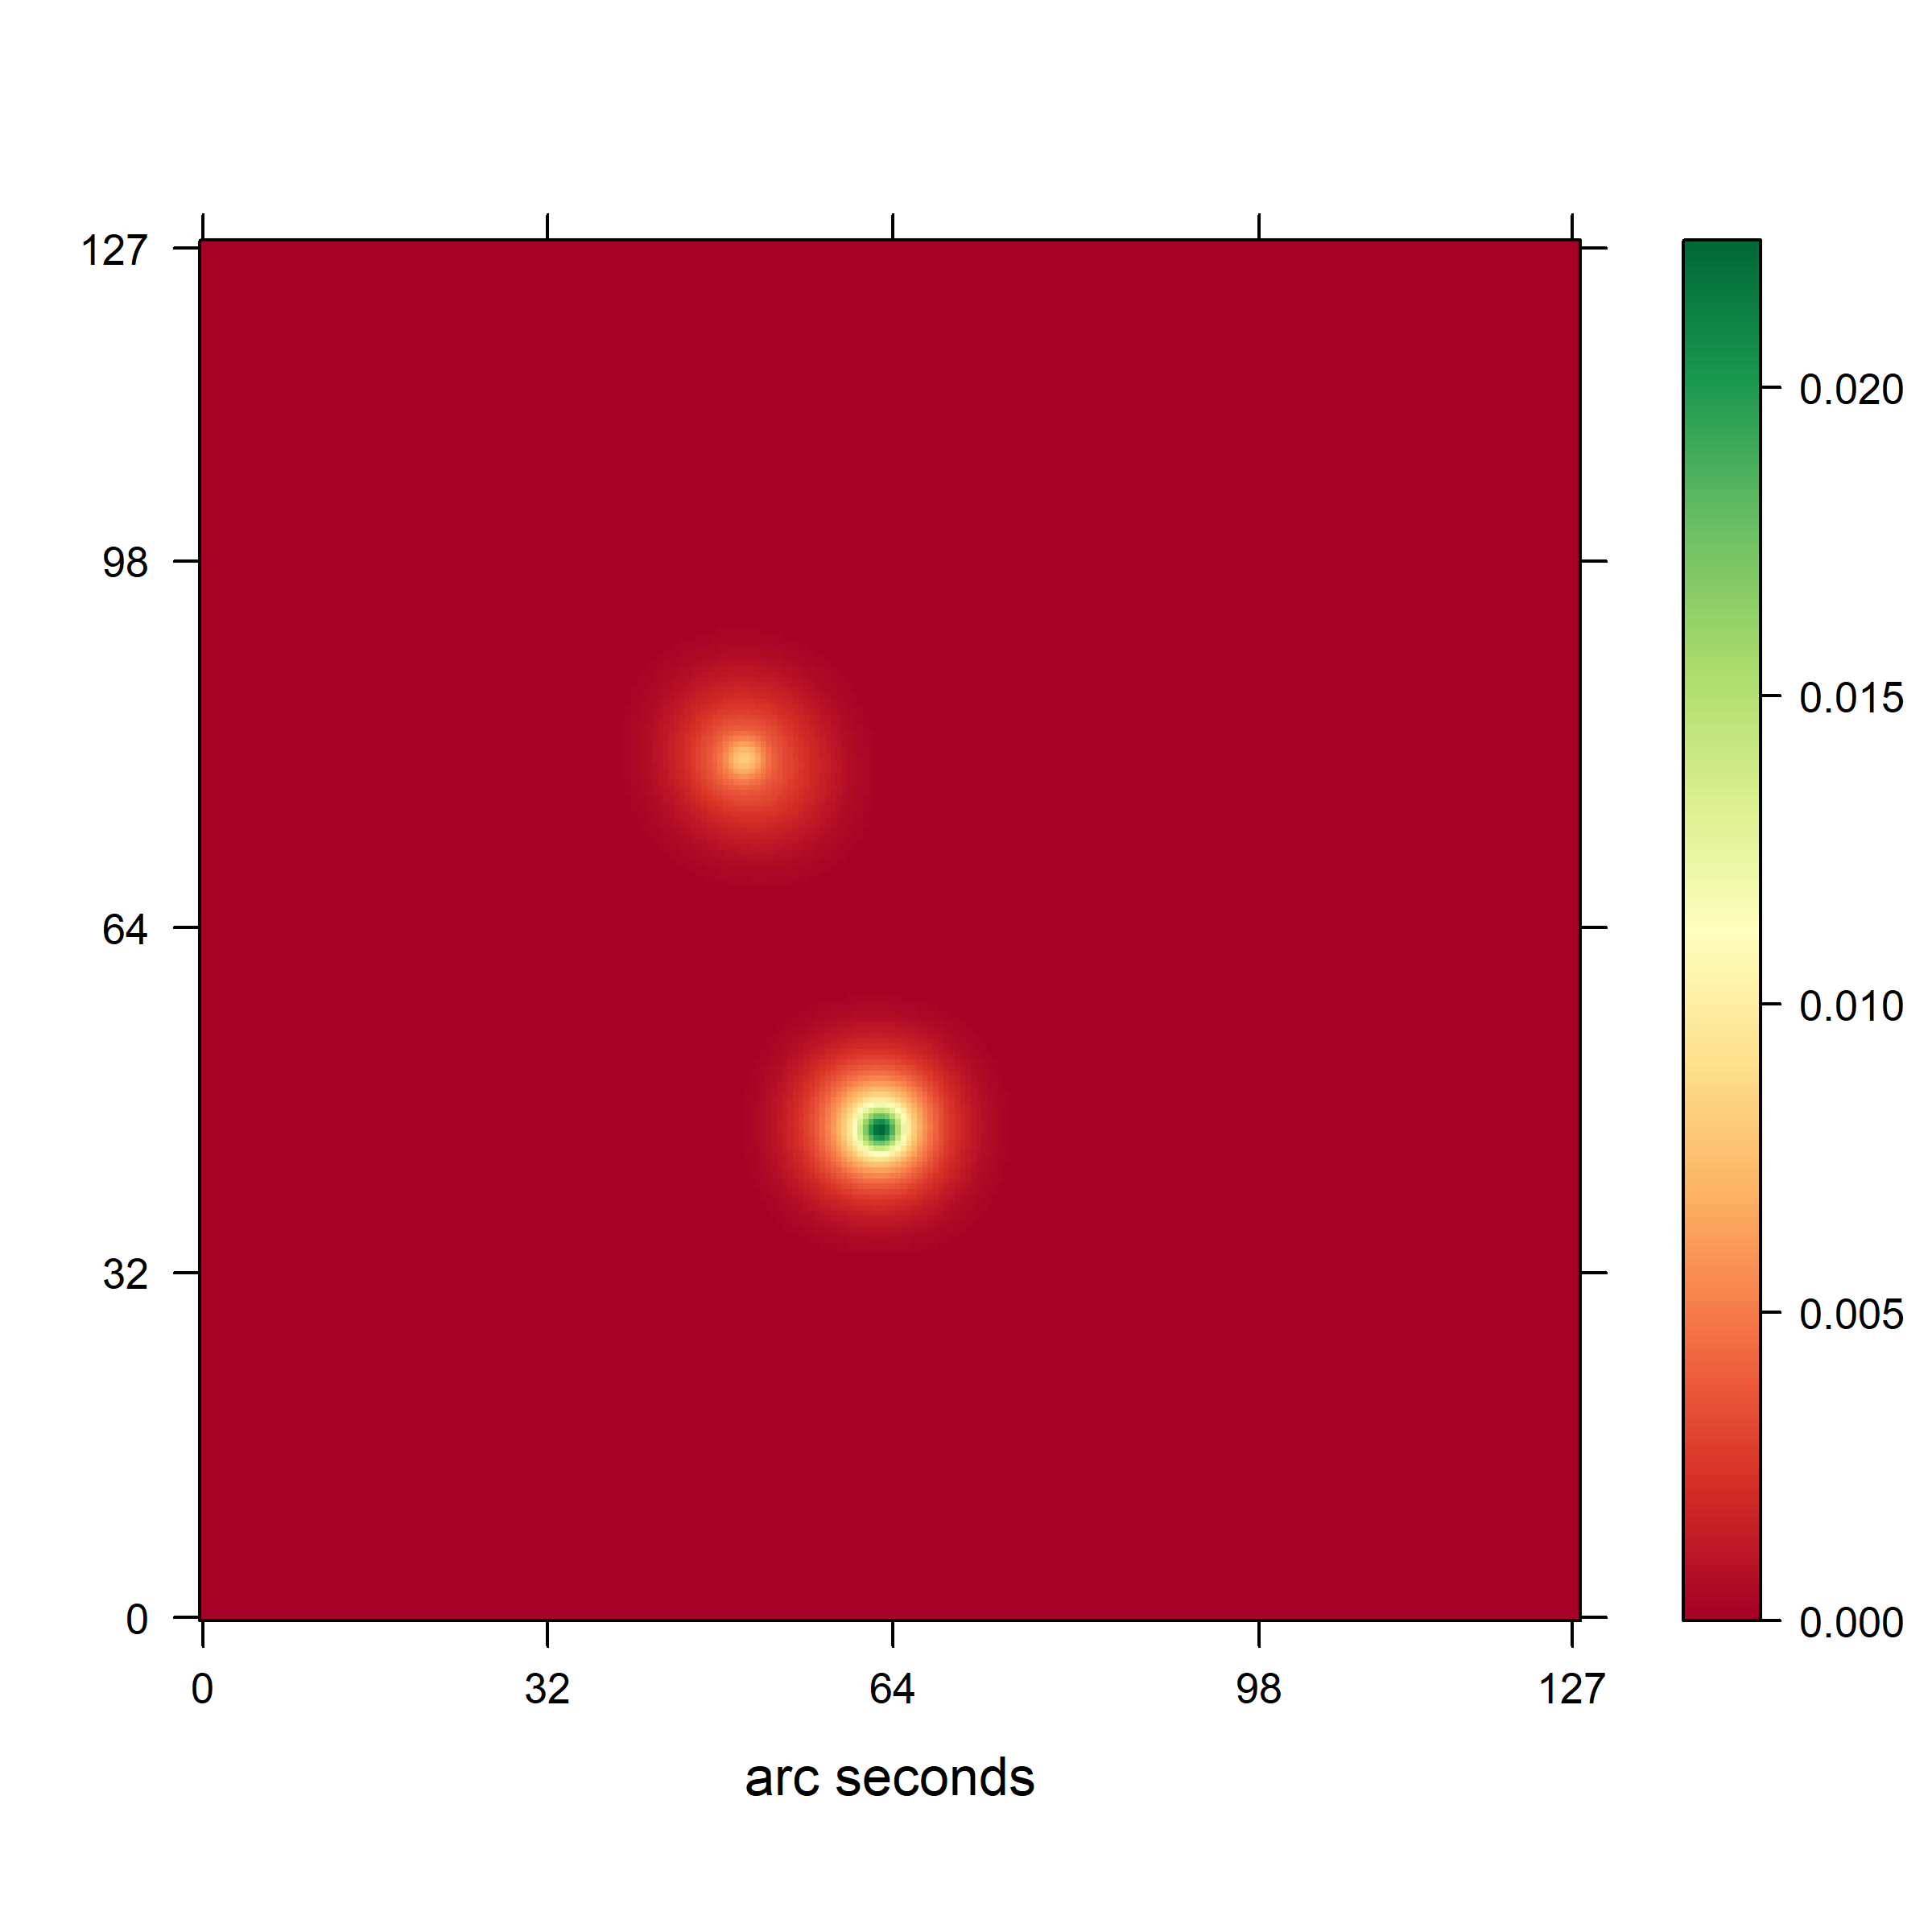
\includegraphics[width=\linewidth, trim={0.2in, 0.2in, 0, 0.2in}, clip]{./chapters/20.results/points/tclean_points.png}
		\caption{CLEAN reconstruction \\with CASA standard parameters.}
		\label{results:points:tclean}
	\end{subfigure}
	\begin{subfigure}[b]{0.4\linewidth}
		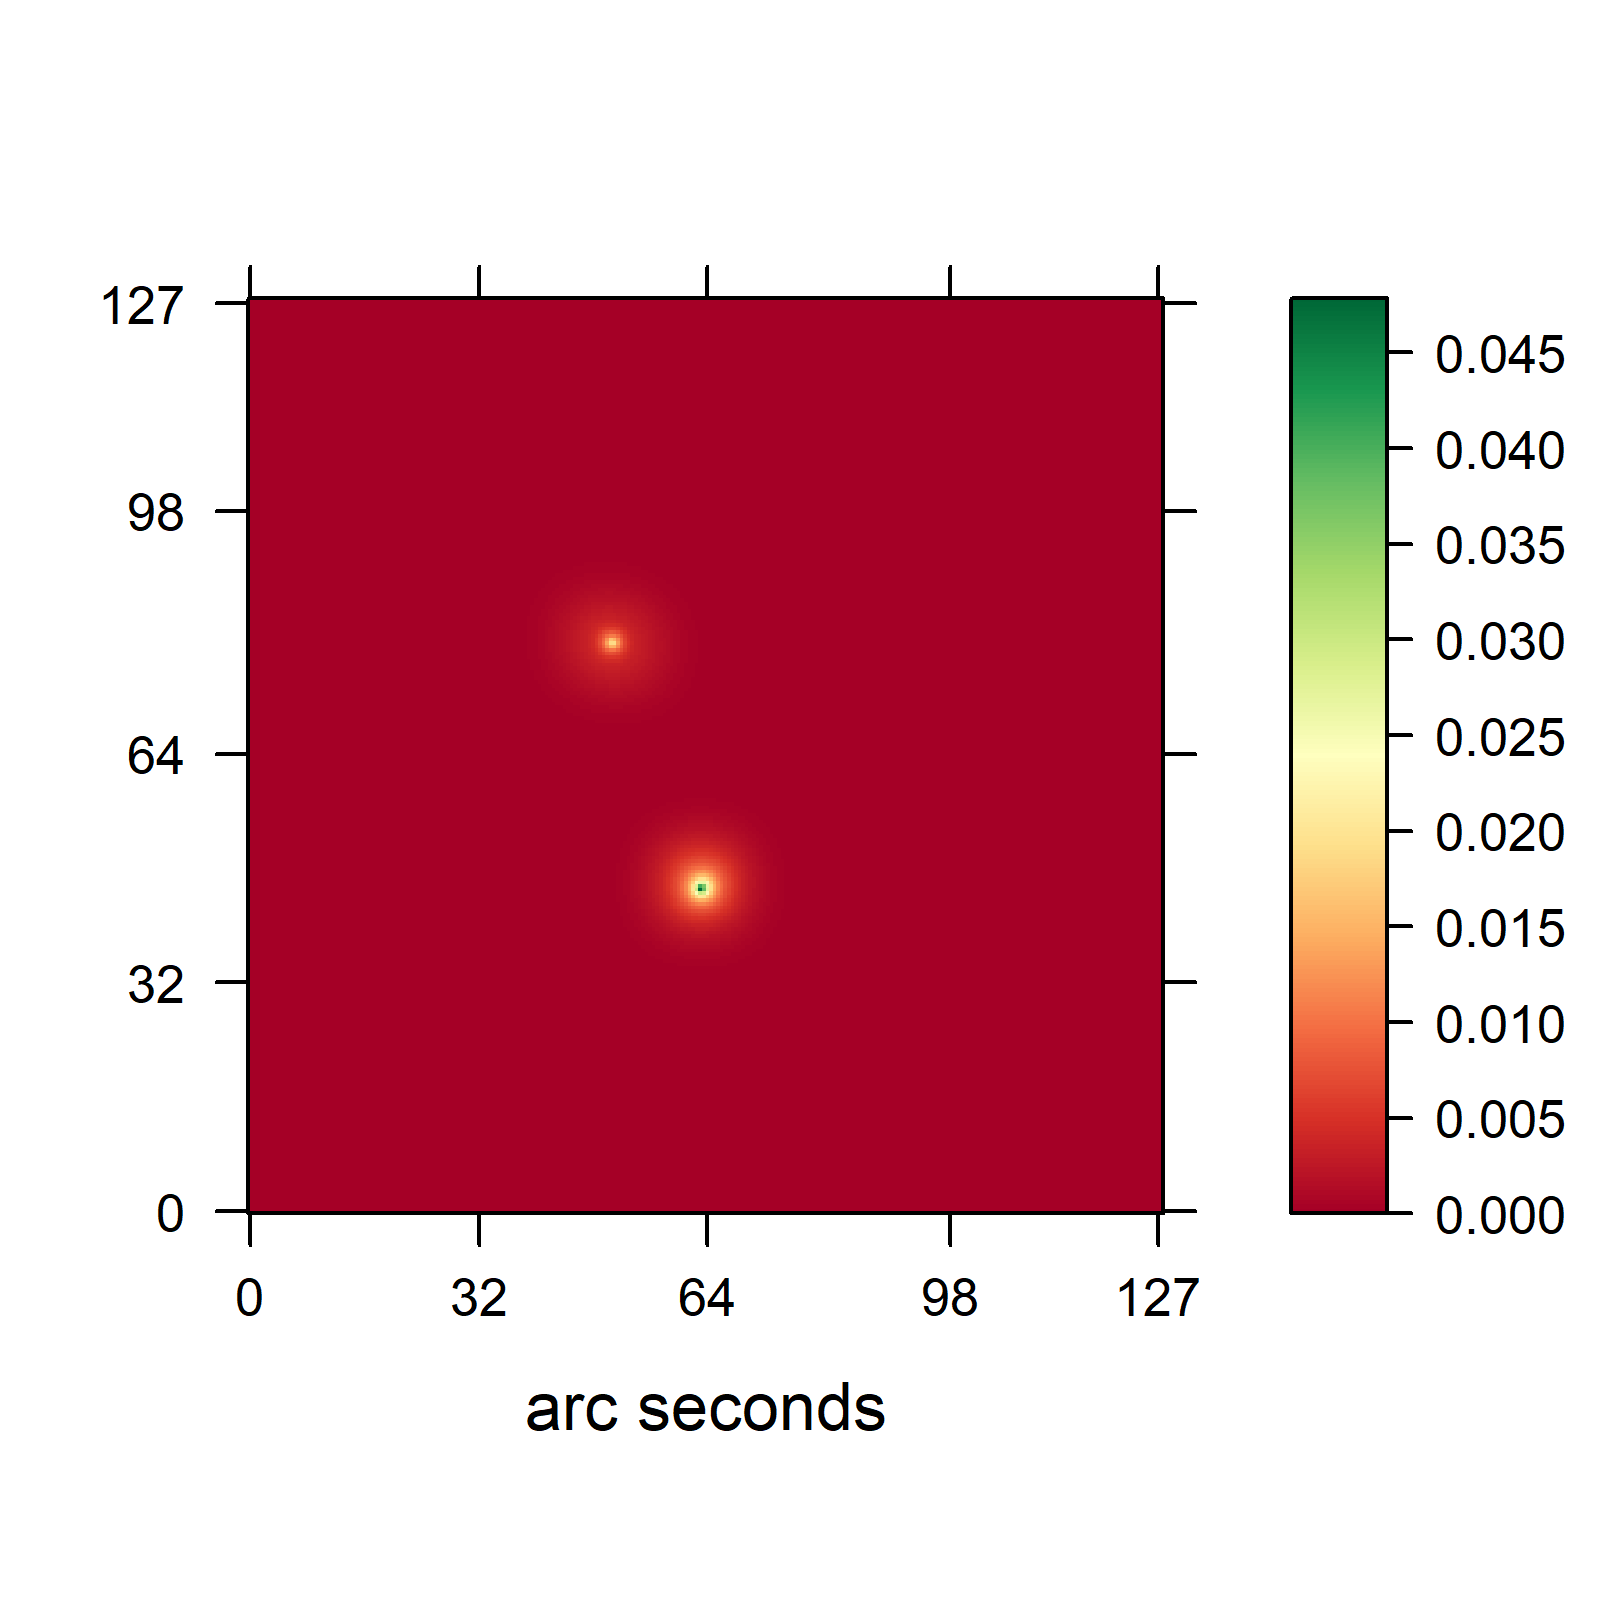
\includegraphics[width=\linewidth, trim={0.2in, 0.2in, 0, 0.2in}, clip]{./chapters/20.results/points/cd_points.png}
		\caption{Coordinate Descent reconstruction\\ with $\lambda = 0.01, J=4$.}
		\label{results:points:cd}
	\end{subfigure}
	
	\caption{Image reconstruction of two point sources.}
	\label{results:points}
\end{figure}

The total Flux of the image, the sum of all emissions, is 3.9 Jansky/Beam in this simulation. CLEAN reconstructs the right peak intensities, both ending up at 2.5 and 1.4 respectively. Since CLEAN reconstructs a blurred version, the total Flux of the image is off by magnitudes. Figure \ref{results:points:contour} compares the intensity profile of CLEAN, Coordinate Descent and the Ground Truth. Note the logarithmic y scale. For a correct total flux, the integrals should be equal. 

\begin{figure}[h]
	\centering
	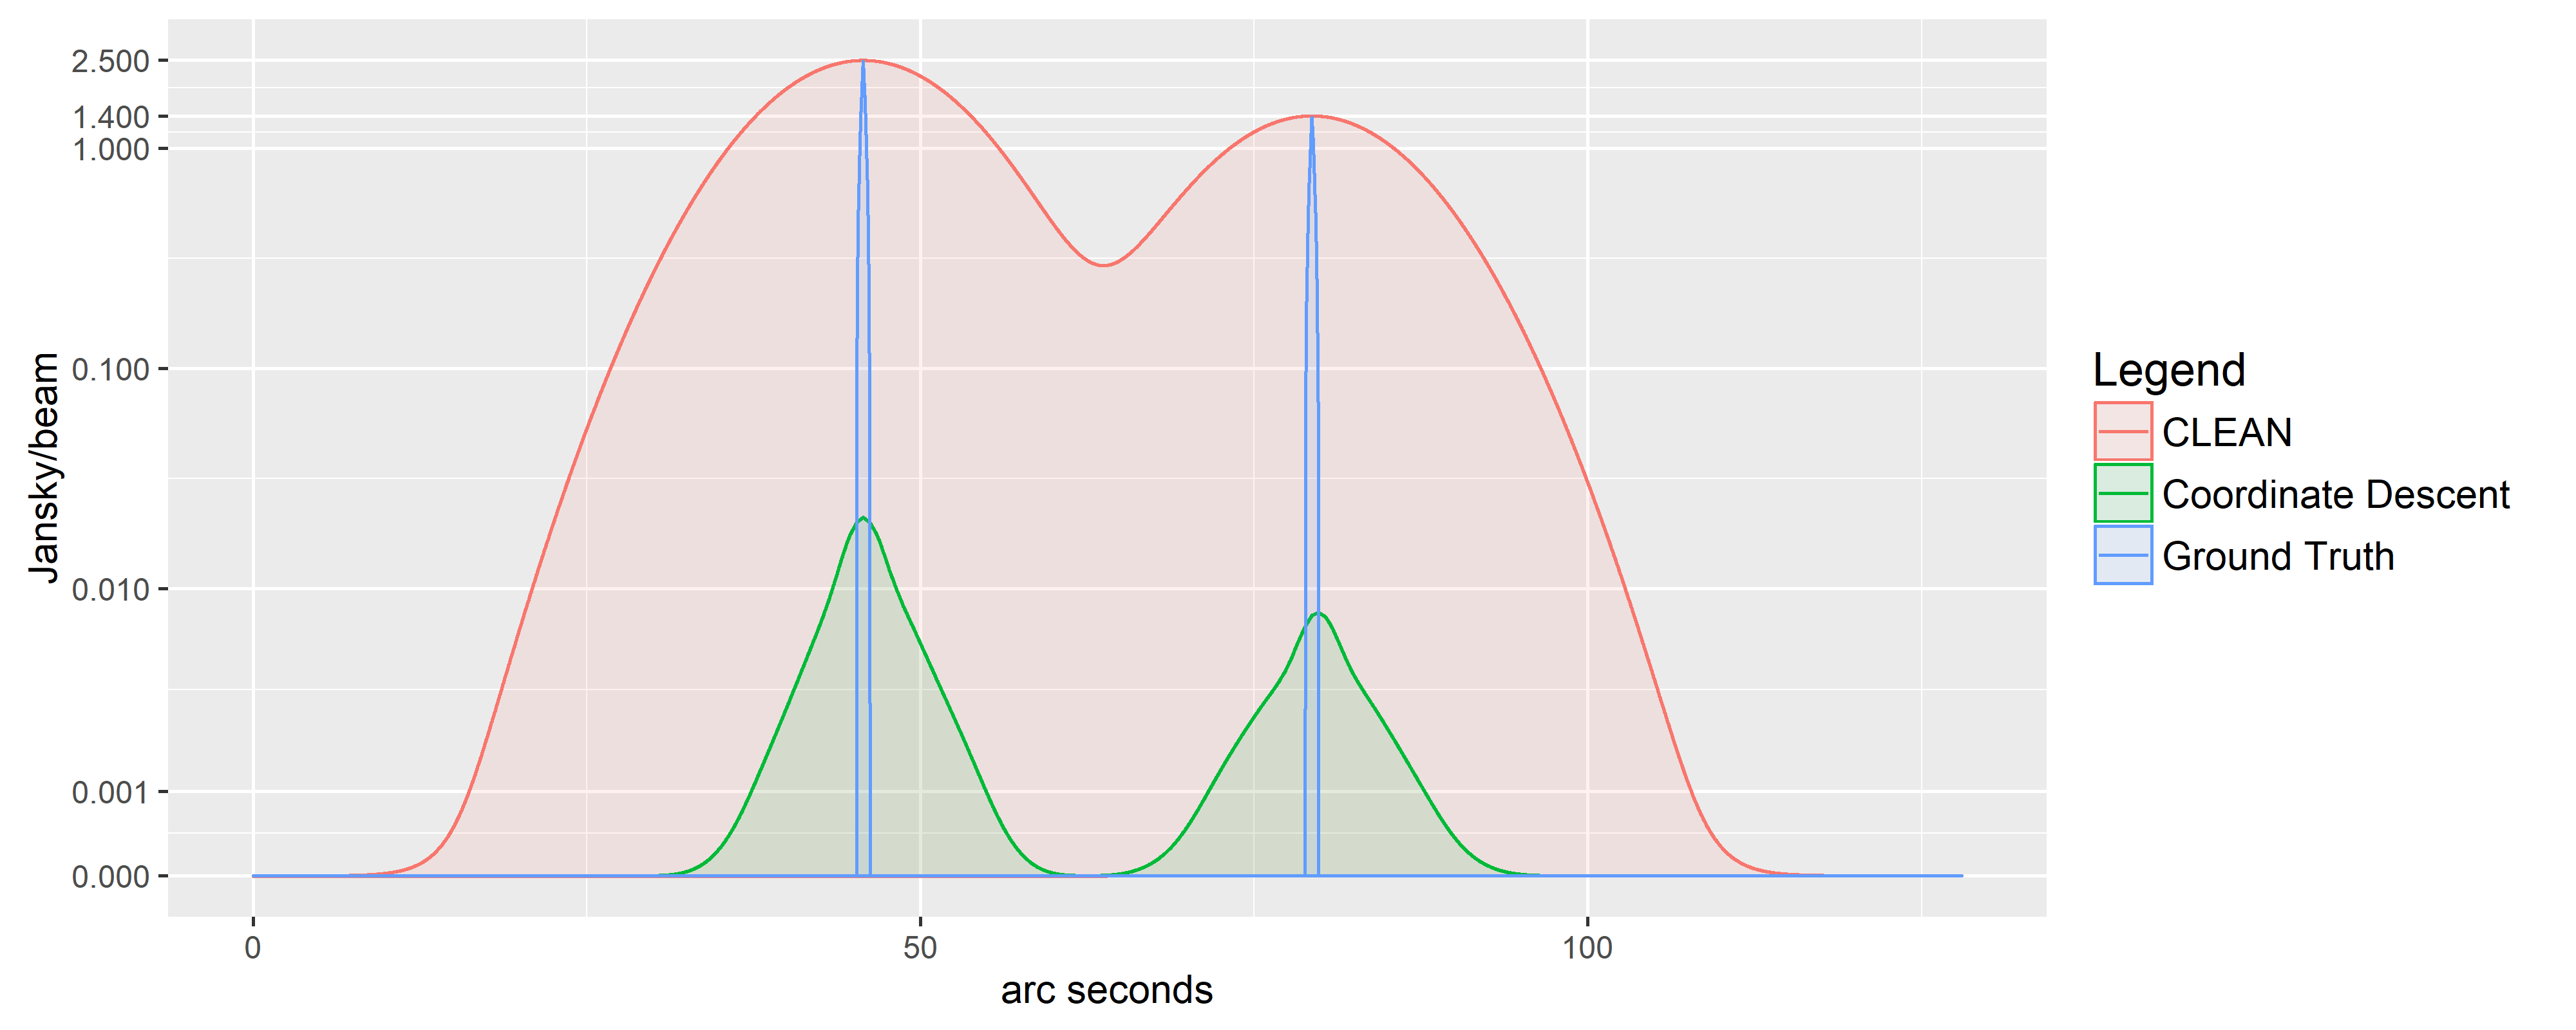
\includegraphics[width=0.8\linewidth]{./chapters/20.results/points/contour_points.png}
	\caption{Intensity profile of the two point sources.}
	\label{results:points:contour}
\end{figure}

In the contour plot, the Coordinate Descents narrow contours become apparent.

The flux is sadly not correct, it seeems to be too large by a factor of two

The larger source was well reconstructed. The second, smaller emissions however has a few issues.

note that the smaller emission is shifted by a pixel and the contour is wider than it's larger cousin. 

The last issue it has that the flux is still not correct. It is close and seems to bigger than a factor of two.



Look at the flux in a more complex environment


\subsection{Super resolution of mixed sources}

Dataset of three gaussian extended emissions and sixteen point sources at varying intensities.

Parameters of Coordinate Descent

super resolution of CD. However, it did not find all point sources
Lets look closer at the flux reconstruction of extended emissions

\begin{figure}[h]
	\centering
	\begin{subfigure}[b]{0.4\linewidth}
		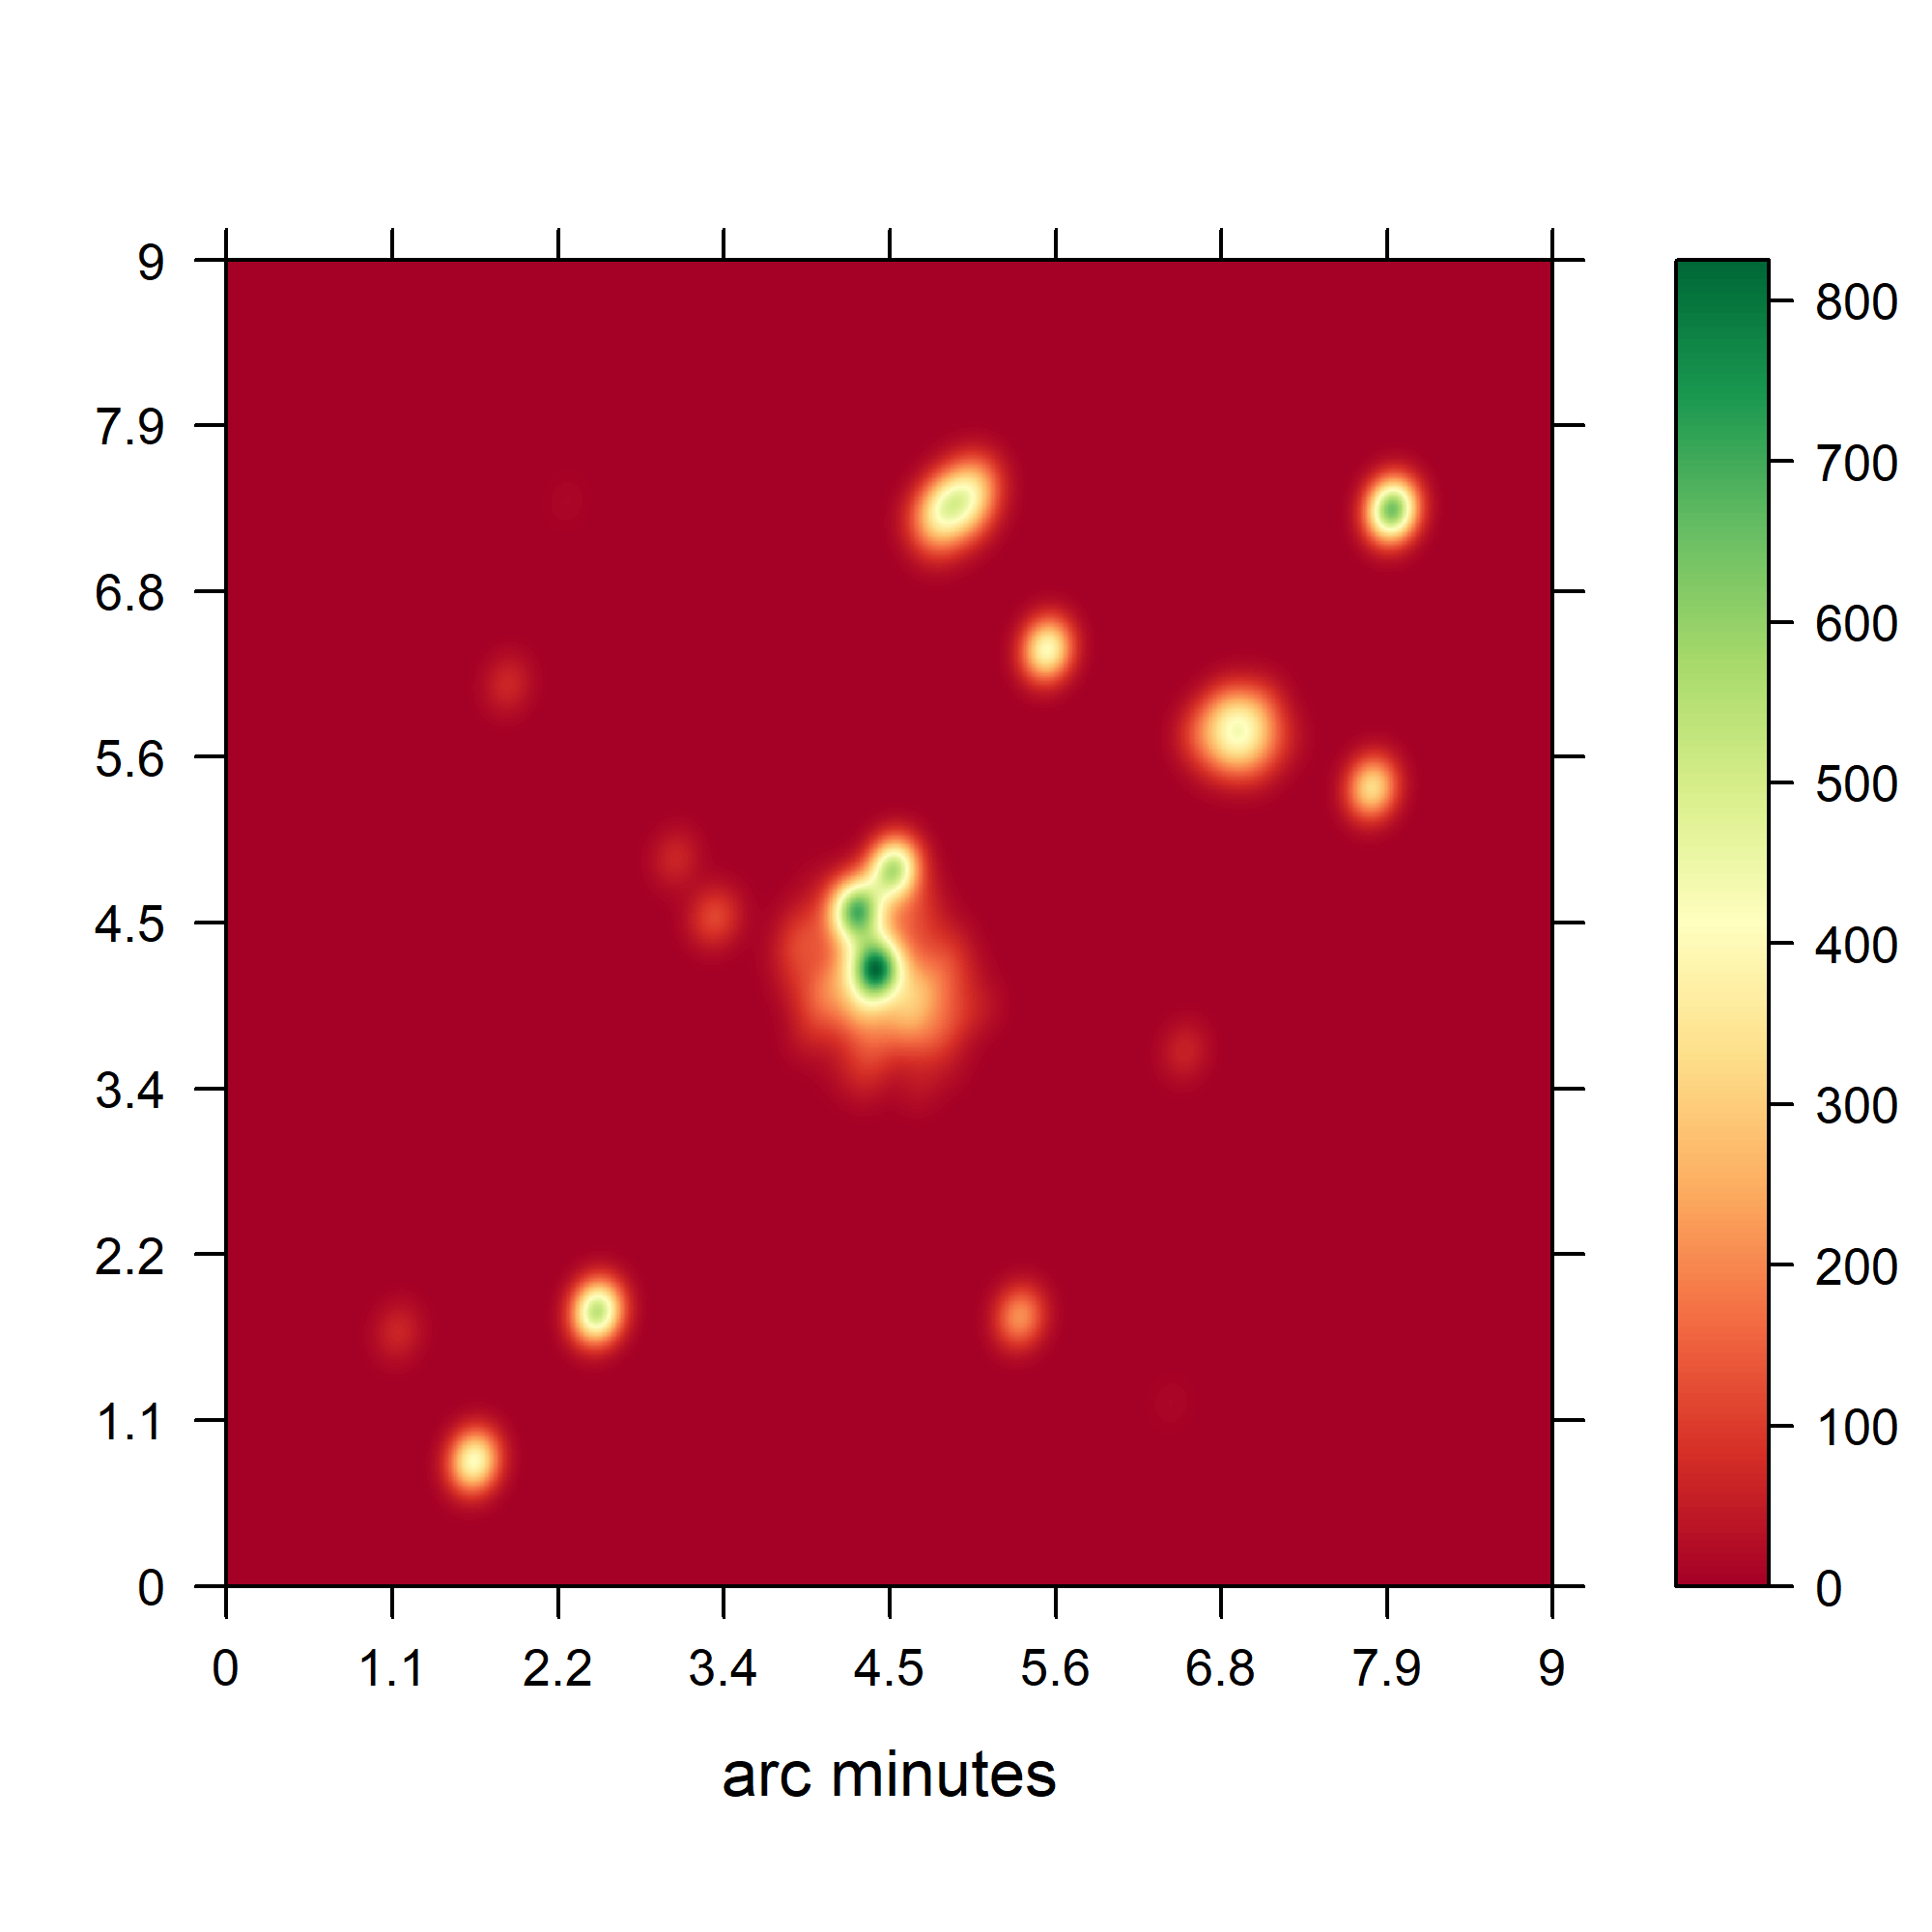
\includegraphics[width=\linewidth, trim={0.2in, 0.2in, 0, 0.2in}, clip]{./chapters/20.results/mixed/mixed_clean.png}
		\caption{CLEAN reconstruction}
		\label{results:mixed:tclean}
	\end{subfigure}
	\begin{subfigure}[b]{0.4\linewidth}
		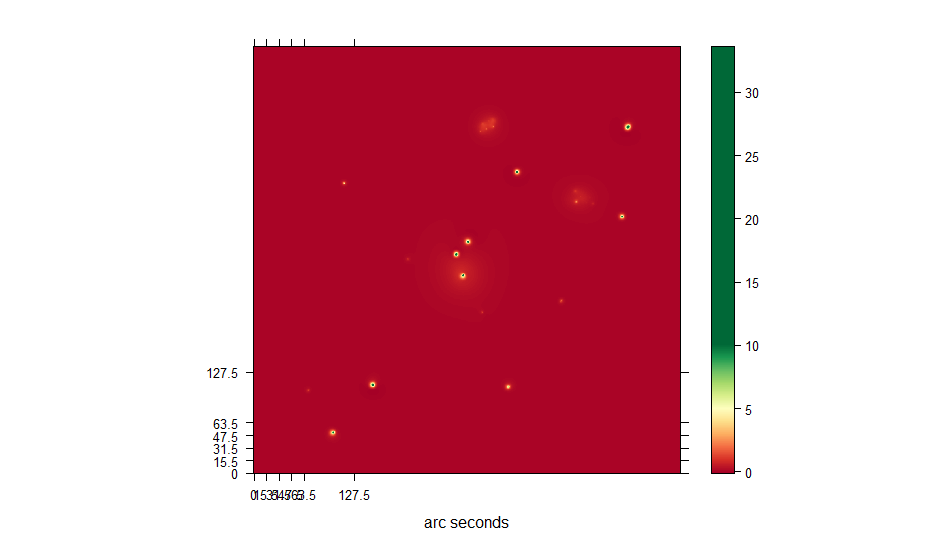
\includegraphics[width=\linewidth, trim={0.2in, 0.2in, 0, 0.2in}, clip]{./chapters/20.results/mixed/mixed_cd.png}
		\caption{Coordinate Descent Reconstruction}
		\label{results:mixed:cd}
	\end{subfigure}
	\caption{Reconstruction on mixed sources}
	\label{results:mixed}
\end{figure}

Question of Flux reconstruction

 $\lambda$ for different starlet layers like in \cite{girard2015sparse}

\begin{figure}[h]
	\centering
	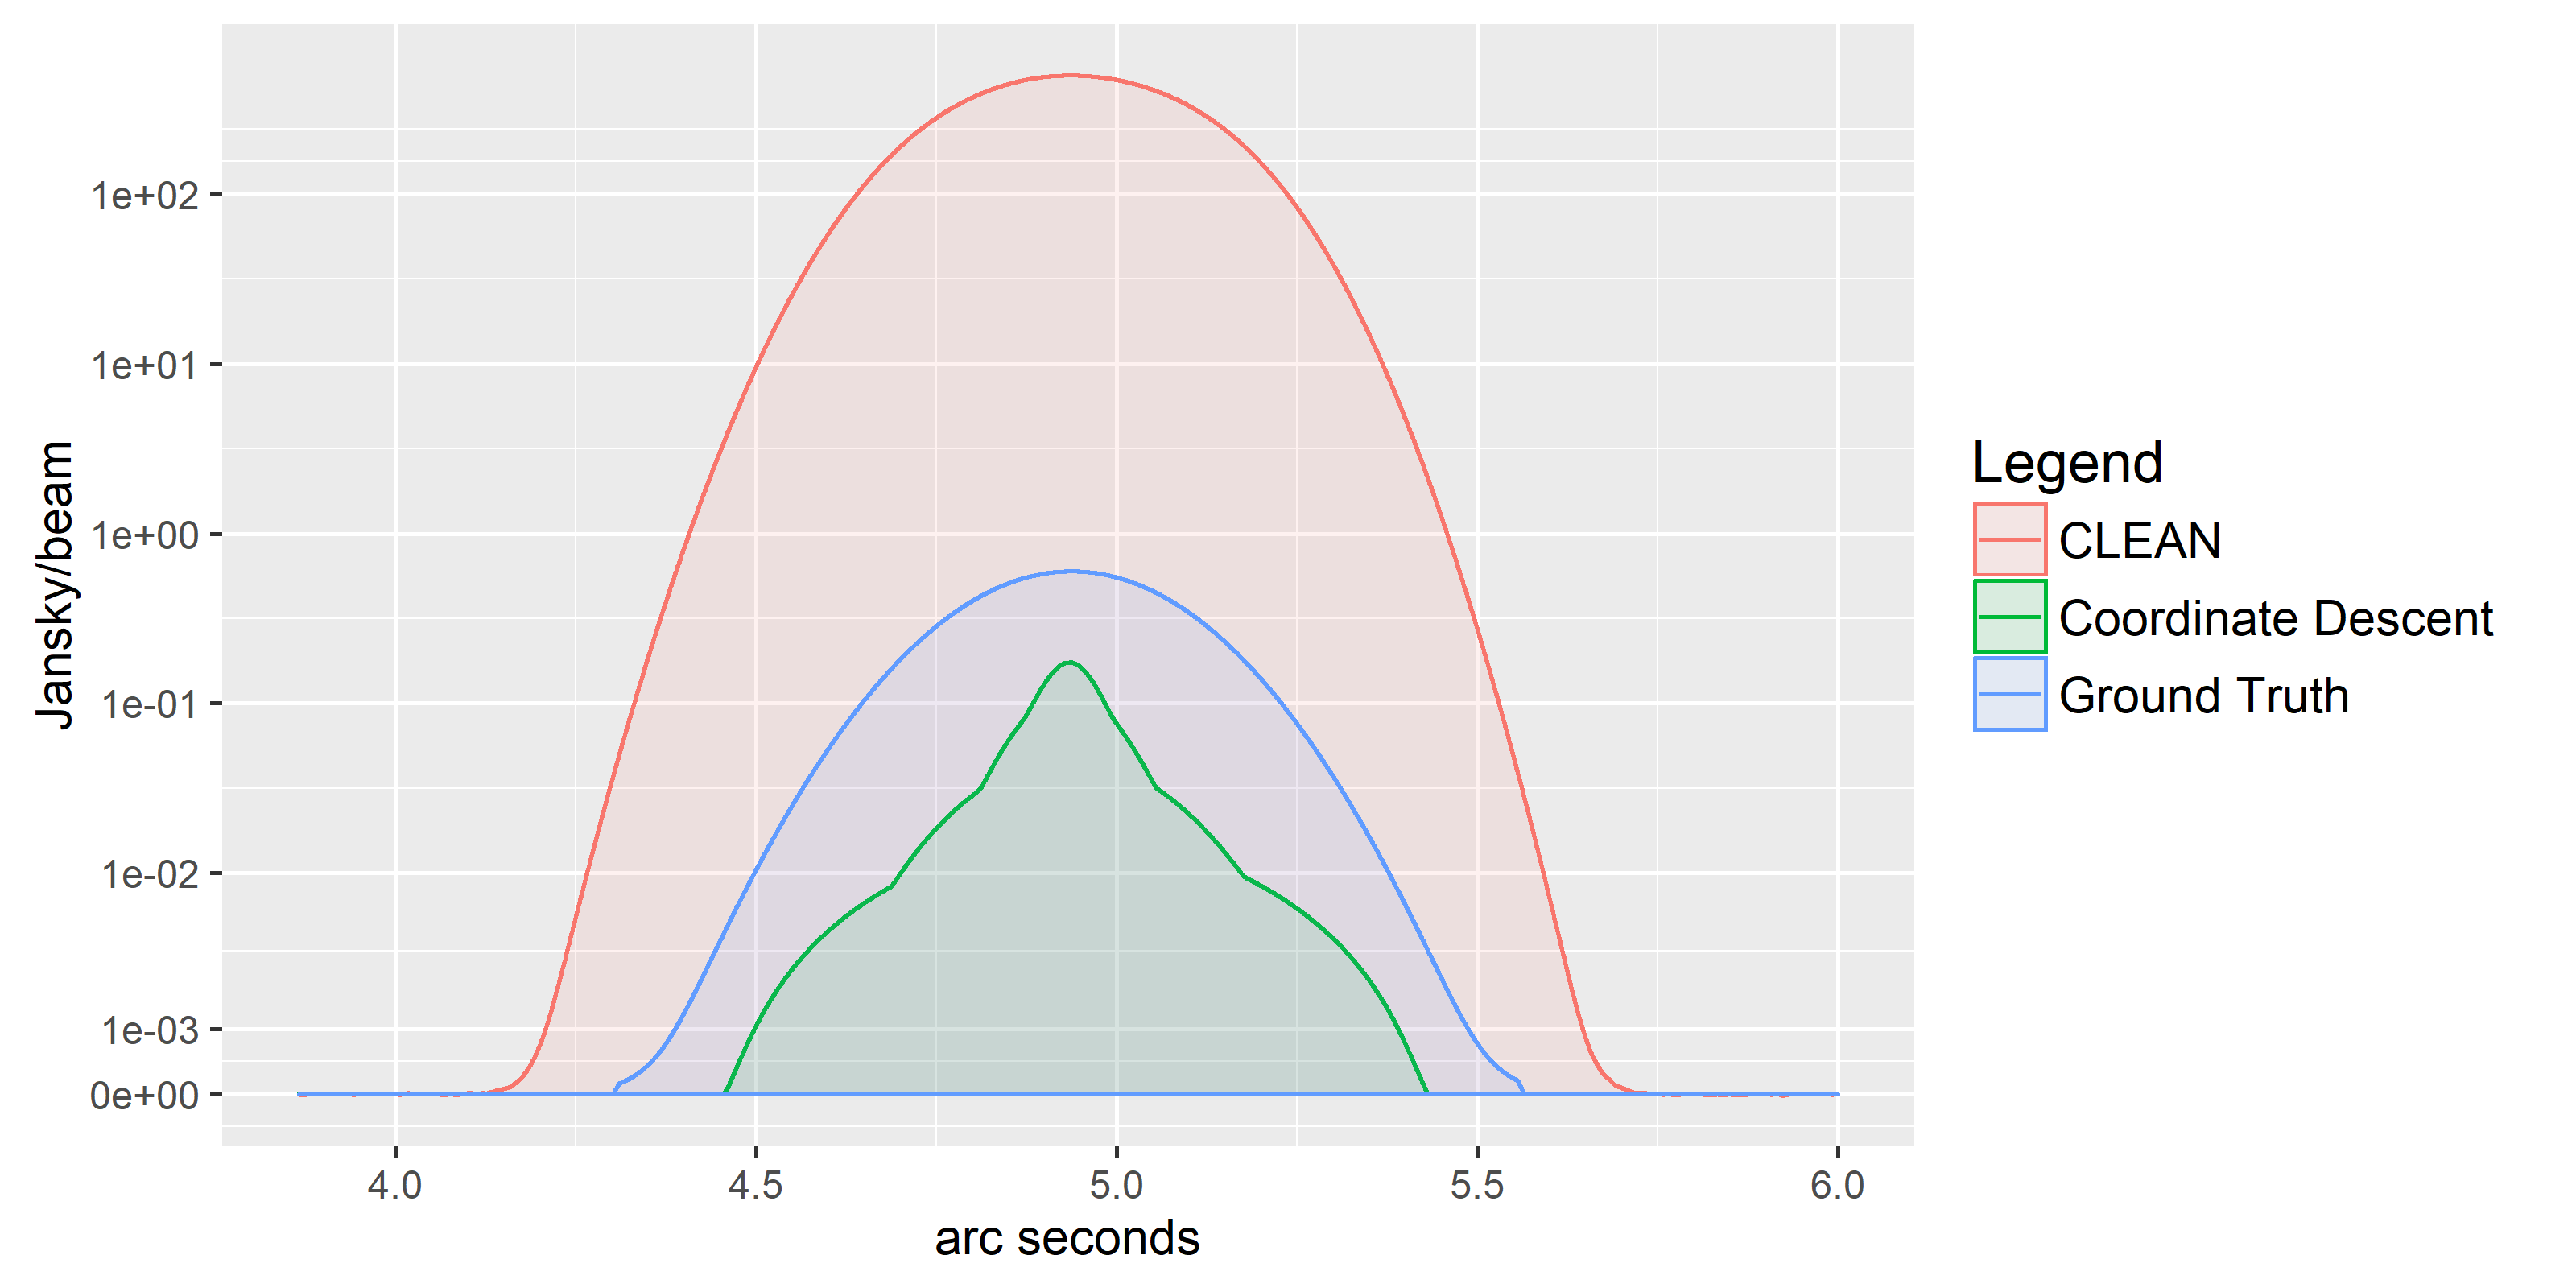
\includegraphics[width=0.8\linewidth]{./chapters/20.results/mixed/mixed_cut0.png}
	\caption{Reconstruction on mixed sources}
	\label{results:mixed:contour}
\end{figure}

Coordinate Descent did not reconstruct all point sources. How many starlets are non-zero is the major point for runtime. It depends on how many areas of the image are non-zero. Starlet has a representation for extended emission, how many starlets are needed for modelling is hard.

Runtime problems
1900 non-zero starlets, 


